%!TEX root = ./main.tex







\section{Tool}
\tool{} contains two major components to it:
%
\begin{itemize}
\item 
Debugging the code
\item
Learning how to code
\end{itemize}
%
The debugging aspect aims to give novices a useful and concise means of evaluating their code.
%
The novice will be able to determine if what they expect the output to be at a certain stage of execution matches what the tool does.
%
The learning aspect will allow lectures and professors the ability to create assignments, such as TopCoder\footnote{https://www.topcoder.com/}.
%
These assignments will allow the professors to gauge where their students are at and see what they are struggling with.
%
The tool will be built as a website application using AngularJS as a framework.
%
By making the tool a website based application, no one wanting to use the tool will have to download anything.
%
The application will include: a space to view the registers, a separate space to view the stack, and a place to write and run code.
%
The code will be viewed using Monaco \footnote{https://microsoft.github.io/monaco-editor/index.html}, a free and open source code editor developed by Microsoft.



\subsection{Debugging The Code}

\begin{figure}[!t]
    \centering
    \vspace{-4pt}
    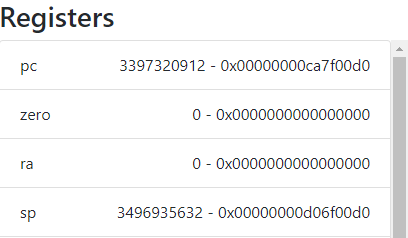
\includegraphics[scale=0.80]{figures/fig-registers.png}
    \caption{Visual Representation of Registers}
    \label{fig-registers}
\end{figure}

There are several options available that help one write and debug their code.
%
Figure \ref{fig-registers} shows the display of the registers.
%
Each register will be listed, accompanied by its value both in decimal and hexadecimal.
%
The user can change a setting determining whether only one of the values should be shown, or both.
%
Important registers, such as the program counter and the stack pointer, will be prioritized and always shown at the top.
%
Other general use registers, such as a0 through a6, will be viewable by scrolling to the bottom of the list.
%
This will allow anyone using the tool to see what the value is at a register at any given time during the breakpoint.


\begin{figure}[!t]
    \centering
    \vspace{-4pt}
    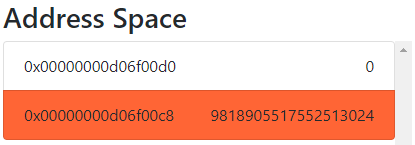
\includegraphics[scale=0.80]{figures/fig-stack.png}
    \caption{Visual Representation of Stack}
    \label{fig-stack}
\end{figure}

Figure \ref{fig-stack} displays the status of the stack as the program continues to be executed.
%
The stack displays the memory address and the value at that memory address, similar to the registers.
%
The current value of the stack pointer register is highlighted.


\begin{figure}[!t]
    \centering
    \vspace{-4pt}
    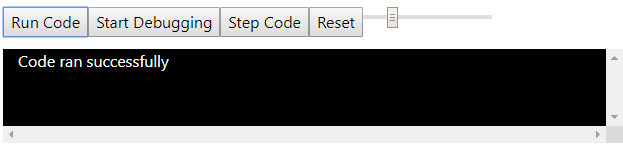
\includegraphics[scale=0.55]{figures/fig-console.png}
    \caption{Output Console}
    \label{fig-console}
\end{figure}


Figure \ref{fig-console} shows where the output of the program will be displayed.
%
In addition to any output from the program, this is where any errors will be shown as well.
%
For example, if an unknown command is written somewhere in the code, it will be shown here.
%
In addition, is a button "Run Code", which will run through the code at a speed determined by the slider to the far right.
%
Initially, each line is ran through at an increment of 0.25 seconds, but can be changed up to 5 seconds and as little as 0 seconds.
%
There is also a "Start Debugging" button, which will allow the code to be incrementally stepped through, such as going through breakpoints in GDB.
%
Finally, the "Stop Code" button will stop the code from running, whether it be the first or second button that is pressed.


Both of these will update in real time as the code is being ran on the application.
%
An option to "step" through the code one line at a time is also available, so having the memory update as the code runs is preferred.
%




\subsection{Learning How To Code}
The tool will also include a spot that will allow instructors to upload assignments that their students can do.
%
The instructor must provide tests that will be ran against the code to make sure that the output matches.
%
This will be similar to TopCoder (mentioned above).
%
The 